%============================================================================
% CCM Tools Manual
%=============================================================================

\documentclass[12pt]{book}

\usepackage[latin1]{inputenc}
\usepackage{listings}


% PDF Document Info
\expandafter\ifx\csname pdfoutput\endcsname\relax
    \usepackage[draft]{hyperref}
    \usepackage{graphicx}
    \DeclareGraphicsExtensions{.eps,.fig}
\else
    \usepackage{hyperref}
    \hypersetup{
        pdfauthor={Egon Teiniker},
        pdftitle={CCM Tools Manual},
        pdfsubject={CORBA Component Model Tools},
        pdfkeywords={CCM, CORBA, components}
    }
    \pdfcompresslevel=9
    \usepackage[pdftex]{graphicx}
    \DeclareGraphicsExtensions{.pdf,.png,.gif,.jpg}
\fi


\setlength{\textwidth}{15 true cm}
\setlength{\textheight}{22 true cm}
\oddsidemargin  0.5 cm
\evensidemargin 0.5 cm
\topmargin      0 cm
\setlength{\parindent}{0cm}

\setcounter{tocdepth}{5} 


\begin{document}
%=Content====================================================================== 
	\pagenumbering{roman}
	\begin{titlepage}

\centering

\vspace*{20mm}
{\huge ccmtools.sourceforge.net }
\vspace{20 mm}

\centerline{\includegraphics[width=40mm]{figures/LocalAdapterConcept.eps}}

\vspace{30mm}

{\Huge CCM Tools IDL }\\ 
\vspace{5mm}
{\bf Egon Teiniker <egon.teiniker@salomon.at>}\\
\vspace{30mm}


{\Large Version: 1.0.0} \\
\vspace{5mm}
$Id$
\end{titlepage}
	\tableofcontents
	\pagenumbering{arabic}

	% $Id$
%==============================================================================
\section{Introduction}
\label{section:Introduction}
%==============================================================================

\dots

\begin{lstlisting}[language=Java]
try
{
    // code
}
catch(...)
{
}
final
{
}
\end{lstlisting}

\begin{lstlisting}[language=C++]
try
{
    // code
}
catch(...)
{
}
\end{lstlisting}


\begin{lstlisting}[language=IDL]
interface IFace
{
	long foo(in string s);
};
\end{lstlisting}
	
	%==============================================================================
\chapter{Hello World Example}
\label{HelloWorldComponent}
%==============================================================================

As a quick tour through CCM Tools, we implement a simple Hello World 
component example. 
Each development step and developer role will be described 
in more detail in one of the next sections, here we give a general overview.

\vspace{5mm}
\noindent
{\bf Step 1:} We define a component using the 
{\it Interface Definition Language} (IDL). 
This simple component only provides a single interface containing a single
method. Don't forget to define a home for this component type.
The following IDL definitions are stored in
a file called {\tt Hello.idl}:
\begin{small}
\begin{verbatim}
module world
{ 
    interface Hello 
    { 
        string sayHello(); 
    }; 

    component Server 
    { 
        provides Hello hello;
    }; 

    home ServerHome manages Server
    {
    };
};
\end{verbatim}
\end{small}


\noindent
{\bf Step 2:} Generate a uniform IDL3 structure from the single {\tt Hello.idl}
file:
\begin{small}
\begin{verbatim}
> ccmidl -idl3 -o server/idl idl3/Hello.idl
\end{verbatim}
\end{small}

\noindent
This uniform IDL3 structure separates between interfaces (including 
parameter type and exception definitions) and components (including their
homes). Such a separation makes sense because an interface can be used by
many component definitions.
\begin{small}
\begin{verbatim}
    server/
     |-- idl
     |   |-- component
     |   |   `-- world
     |   |       |-- Server.idl
     |   |       `-- ServerHome.idl
     |   `-- interface
     |       `-- world
     |           `-- Hello.idl
\end{verbatim}
\end{small}


\noindent
{\bf Step 3:} Generate an empty component skeleton from the uniform IDL3 
structure:
\begin{small}
\begin{verbatim}
> ccmtools c++local -o server/interface \
                    -Iserver/idl/interface \
                    -Iserver/idl/component \
                    server/idl/interface/world/*.idl

> ccmtools c++local -a -o server/component/Server \ 
                    -Iserver/idl/interface \
                    -Iserver/idl/component \
                    server/idl/component/world/Server*.idl  
\end{verbatim}
\end{small}

\noindent
CCM Tools generate the following file structure which represents a local
component's implementation.
Code contained in the {\tt GEN\_*} directories establishes the component's
structure (= {\it component logic}), while code stored in the {\tt Server} 
directory represents the functional part of a component (= {\it business
logic}).

\begin{small}
\begin{verbatim}
   server
    |-- idl
    |-- component
    |   `-- Server
    |       |-- GEN_ccmtools_local_world
    |       |-- GEN_ccmtools_local_world_share
    |       |-- ServerHome_impl.cc
    |       |-- ServerHome_impl.h
    |       |-- Server_hello_impl.cc
    |       |-- Server_hello_impl.h
    |       |-- Server_impl.cc
    |       |-- Server_impl.h
    |       `-- world_ServerHome_entry.h
    `-- interface
        |-- GEN_ccmtools_local_world
        `-- GEN_world
\end{verbatim}
\end{small}

\noindent
{\bf Step 4:} Implement the component's business logic.
The component's business logic must be embedded in the generated
component logic. 
To implement the {\tt sayHello()} method of the {\tt Hello} interface,
we extend the generated {\tt Server\_hello\_impl.cc} file:
\begin{small}
\begin{verbatim}
std::string
Server_hello_impl::sayHello()
    throw(Components::CCMException)
{
    // TODO : IMPLEMENT ME HERE !
    return "Hello from Server component!";
}
\end{verbatim}
\end{small}


\noindent
{\bf Step 5:} Now we can implement a client that uses the Hello World
component. For this simple case, we implement the client as a {\tt \_check*}
file that will be automatically executed from a {\tt make check} command.

\begin{small}
\begin{verbatim}
   server/component/server
    |-- test
    |   `-- _check_world_Server.cc
\end{verbatim}
\end{small}

\noindent
The following client code snippets are stored in the 
{\tt \_check\_world\_Server.cc} file:
\begin{small}
\begin{verbatim}
#include <cassert>
#include <iostream>

#include <Components/ccmtools.h>
#include <world/ServerHome_gen.h>

using namespace std;
using namespace world;

int main(int argc, char *argv[])
{
    int error = deploy_world_ServerHome("ServerHome");
    if(error)
    {
        cerr << "BOOTSTRAP ERROR: Can't deploy component homes!" << endl;
        return(error);
    }

    try
    {
        Components::HomeFinder* homeFinder = 
            Components::HomeFinder::Instance();

        ServerHome::SmartPtr home(dynamic_cast<ServerHome*>(
            homeFinder->find_home_by_name("ServerHome").ptr()));

        Server::SmartPtr component;
        Hello::SmartPtr hello;

        component = home->create();
        hello = component->provide_hello();
        component->configuration_complete();

        string s = hello->sayHello();
        cout << "sayHello(): " << s << endl;

        assert(s == "Hello from Server component!");

        component->remove();
    }
    catch(Components::Exception& e)
    {
        cerr << "CCMTOOLS ERROR: " << e.what() << endl;
        return -1;
    }
    catch(...)
    {
        cerr << "UNKNOWN ERROR!" << endl;
        return -1;
    }

    error = undeploy_world_ServerHome("ServerHome");
    if(error)
    {
        cerr << "TEARDOWN ERROR: Can't undeploy component homes!" << endl;
        return error;
    }

    Components::HomeFinder::destroy();
}
\end{verbatim}
\end{small}

\noindent
Additionally, we create some marker files which tell
{\tt confix} which package name, version and subdirectories
should be used.
\begin{small}
\begin{verbatim}
> ccmconfix -confix2 -o server -pname "hello_world" -pversion "1.0.0"
\end{verbatim}
\end{small}

\noindent
To compile the component and run the unit test, simply type: 
\begin{small}
\begin{verbatim}
> confix2.py --packageroot=`pwd`/server --bootstrap --configure \
            --make --targets=check
\end{verbatim}
\end{small}

\noindent
After all, we are happy to see the following output at the end of the client's
build process:

\begin{small}
\begin{verbatim}
sayHello(): Hello from Server component!
PASS: hello_world_component_Server_test__check_world_Server
==================
All 1 tests passed
==================
\end{verbatim}
\end{small}

\noindent
Of course, to implement a component for a simple 'Hello from Server component!'
message is somewhat academical, but this example shows how simple a component
development cycle can be. 
The intent of this section was to define the main activities in component 
development, which are:
\begin{itemize}
\item Define a component's structure using IDL.
\item Generate an empty component skeleton (called component logic).
\item Implement a component's business logic. 
\item Implement a component's (test) client.
\end{itemize}

\noindent
In the following sections, we will explore each of these steps in more
detail. However, keep this big picture in mind. 


	% $Id$
%=============================================================================
\chapter{Interface Definition Language}
\label{chapter:InterfaceDefinitionLanguage}
%=============================================================================

% $Id$
%==============================================================================
\section{Introduction}
\label{section:Introduction}
%==============================================================================

\dots

\begin{lstlisting}[language=Java]
try
{
    // code
}
catch(...)
{
}
final
{
}
\end{lstlisting}

\begin{lstlisting}[language=C++]
try
{
    // code
}
catch(...)
{
}
\end{lstlisting}


\begin{lstlisting}[language=IDL]
interface IFace
{
	long foo(in string s);
};
\end{lstlisting}
\input{InterfaceDefinitionLanguage/SourceFiles}
%=============================================================================
\section{Basic IDL Types}
%=============================================================================
IDL provides a number of build--in basic types. 
The CORBA specification requires that language mappings preserve the {\it size}
of basic IDL types.
To avoid restricting the possible target environments and languages, the 
specification leaves the size and range requirements for IDL basic types loose.


%-----------------------------------------------------------------------------
\subsection{Integer Types}
%-----------------------------------------------------------------------------

\begin{itemize}
  \item {\tt short} (range from $-2^{15}$ to $2^{15}-1$, size $\geq$ 16 bits)
  \item {\tt long} (range from $-2^{31}$ to $2^{31}-1$, size $\geq$ 32 bits)
  \item {\tt unsigned short} (range from $0$ to $2^{16}-1$, size  $\geq$
  16 bits)
  \item {\tt unsigned long} (range from $0$ to $2^{32}-1$, size $\geq$ 32
  bits)
\end{itemize}

%-----------------------------------------------------------------------------
\subsection{Floating--Point Types}
%-----------------------------------------------------------------------------

\begin{itemize}
  \item {\tt float} (IEEE single--precision, size $\geq$ 32 bits)
  \item {\tt double} (IEEE double--precision, size $\geq$ 64 bits)
\end{itemize}


%-----------------------------------------------------------------------------
\subsection{Characters}
%-----------------------------------------------------------------------------
\begin{itemize}
  \item {\tt char} (ISO Latin--1, $\geq$ 8 bits)
  \item {\tt wchar} ($\geq$ 16 bits)
\end{itemize}

%-----------------------------------------------------------------------------
\subsection{Strings}
%-----------------------------------------------------------------------------
\begin{itemize}
  \item {\tt string} (ISO Latin--1, variable--length)
  \item {\tt wstring} (variable--length)
\end{itemize}

%-----------------------------------------------------------------------------
\subsection{Booleans}
%-----------------------------------------------------------------------------
Boolean values can have only the values {\tt TRUE} and {\tt FALSE}. 

%-----------------------------------------------------------------------------
\subsection{Octets}
%-----------------------------------------------------------------------------
The IDL type {\tt octet} is an 8--bit type that is guaranteed not to undergo any
changes in representation as it is transmitted between processes.

%-----------------------------------------------------------------------------
\subsection{Type any}
%-----------------------------------------------------------------------------
Type {\tt any} is a universal container type. A value of type {\tt any} can hold
a value of any other IDL type (e.g. {\tt long}, {\tt string}, or even another
value of type {\tt any}).
Type {\tt any} is useful when you don't know at compile time what IDL types you
will eventually need to transmit between client and server, you can find out at
runtime what type of value is contained in the {\tt any}.
It is recommended to use a {\tt typedef} construct to introduce any types in your
interface definition files. 

\vspace{2mm}
Example:
\begin{verbatim}
    typedef any GenericType;
\end{verbatim}
  

%=============================================================================
\section{User--Defined IDL Types}
%=============================================================================
In addition to providing the build--in basic types, IDL permits you to define
complex types: enumerations, structures and sequences. You can also use {\tt 
typedef} to explicitly name a type.
\vspace{5mm}


%-----------------------------------------------------------------------------
\subsection{Named Types}
%-----------------------------------------------------------------------------

You can use {\tt typedef} to create a new name for a type or to rename an
existing type.

\vspace{2mm}
Example:
\begin{verbatim}
    module world
    {
        typedef long TimeStamp;
    }; // end of module world
\end{verbatim}

Be careful about the semantics of IDL {\tt typedef}. It depends on the language
mapping whether an IDL {\tt typedef} results in a new, separate type or only an
alias. 
To avoid potential problems, you should define each logical type exactly once
and then use that definition consistently throughout your specification.


%-----------------------------------------------------------------------------
\subsection{Enumerations}
%-----------------------------------------------------------------------------
An IDL enumerated type definition looks much like the C++ version.

\vspace{2mm}
Example:
\begin{verbatim}
    module world
    {
        enum Color 
        {
            red, 
            green, 
            blue
        };
    }; // end of module world
\end{verbatim}

This example introduces a type named {\tt Color} that becomes a new type in its
own right - there is no need to use a {\tt typedef} to name the type.


%-----------------------------------------------------------------------------
\subsection{Structures}
%-----------------------------------------------------------------------------
IDL supports structures containing one or more named members of arbitrary type,
including user--defined complex types.

\vspace{4mm}
Example:
\begin{verbatim}
    module world
    {
        struct TimeOfDay
        {
            short hh;
            short mm;
            short ss;
        };
    }; // end of module world
\end{verbatim}

This definition introduces a new type called {\tt TimeOfDay}.
Structure definition form a namespace, so the names of the structure members
need to be unique only within their enclosing structure.

%-----------------------------------------------------------------------------
\subsection{Sequences}
%-----------------------------------------------------------------------------
Sequences are variable--length vectors that can contain any element type. 

\vspace{2mm}
Example:
\begin{verbatim}
    module world
    {
        typedef sequence<Color> Colors; 
    }; // end of module world
\end{verbatim}

A sequence can hold any number of elements up to the memory limits of your
platform. 

\vspace{5mm}


% $Id$
%=============================================================================
\section{Modules}
%=============================================================================
IDL uses the {\tt module} construct to create namespaces.
Modules combine related definitions into a logical group and prevent pollution
of the global namespace.

Identifiers in a module need be unique only within that module.
Modules do not hide their contents, so you can use a type defined in one module
inside another module.

Modules can contain any definition that can appear at global scope.
In addition, modules can contain other modules, so you can create nested
hierarchies. 

Modules can be reopened. 
Incremental definition of modules is useful if specifications are written by a
number of developers (instead of creating a giant definition inside a single
module, you can break the module into a number of separate source files).


\newpage
%=============================================================================
\section{Interfaces}
%=============================================================================

The focus of IDL is on interfaces and operations. 
IDL interfaces define only the interface to an object and say nothing about the
object's implementation. This has the following consequences:
\begin{itemize}
\item By definition, everything in an interface is public. 
Things are made private by simply not saying anything about them.

\item IDL interfaces don't have member variables.
Member variables store state, and the state of an object is an implementation
concern.
\end{itemize}

IDL interfaces form a namespace. You can nest the following constructs inside 
an interface: constant definitions, attribute definitions, and operation definitions.

\newpage
Example:
\begin{verbatim}
    module world
    {
        interface IFace
        {
            /** Constant definitions  */
        
            /** Attibute definitions  */
        
            /** Operation definitions */
        };
    }; // end of module world
\end{verbatim}

It is important to note that IDL operations and attributes define the only 
communication path between objects.
The kinds of information traveling along the communication path are the
parameters, return value, and exceptions of an operation.


%-----------------------------------------------------------------------------
\subsection{Constant Definitions}
%-----------------------------------------------------------------------------

IDL permits the definition of constants, thus, you can define floating--point,
integer, character, string, boolean, and octet constants.
IDL does not allow you to define a constant of type {\tt any} nor a user--defined 
complex type.

\vspace{2mm}
Example:
\begin{verbatim}
    module europe
    {
        interface ConstantsTest
        {
            const boolean BOOLEAN_CONST = TRUE;
            const octet OCTET_CONST = 255;
            const short SHORT_CONST = -10;
            const unsigned short USHORT_CONST = 7;
            const long LONG_CONST = -7777;
            const unsigned long ULONG_CONST = 7777;
            const char CHAR_CONST = 'c';
            const string STRING_CONST = "1234567890";  
            const float FLOAT_CONST = 3.14;
            const double DOUBLE_CONST = 3.1415926;        
        };
    }; // end of module europe
\end{verbatim}


%-----------------------------------------------------------------------------
\subsection{Attributes}
%-----------------------------------------------------------------------------

An attribute can be used to create something like a public member variable.
In fact, an attribute defines a pair of operations the client can call to
sent and receive a value.
Note that IDL attributes don't define storage or state.

\vspace{2mm}
Example:
\begin{verbatim}
    module america
    {
        struct Person 
        {
            long id;
            string name;
        };  
    
        interface AttributeInterface
        {
            attribute long longAttr;
            attribute double doubleAttr;
            attribute string stringAttr;
            attribute Person personAttr;
        };
    }; // end of module america    
\end{verbatim}

Attributes can be of any type, including user--defined complex types.


%-----------------------------------------------------------------------------
\subsection{Operations}
%-----------------------------------------------------------------------------

An operation definition can occur only as part of an interface definition, and
must contain:

\begin{itemize}
\item A return result type
\item An operation name
\item Zero or more parameter declarations
\end{itemize}

\vspace{2mm}
Example:
\begin{verbatim}
    module austria
    {
        interface SimpleInterface
        {
            /**
             * This is the simplest possible operation, because
             * op requires no parameters and does not return a value.
             */
            void op(); 
        };
    }; // end of module austria
\end{verbatim}

Notice that a parameter must be qualified with one of three 
{\bf directional attributes}:
\begin{itemize} 
\item {\bf in}\\
	The {\tt in} attribute indicates that the parameter is sent from
	the client to the server.
\item {\bf out}\\
	The {\tt out} attribute indicates that the parameter is sent from 
	the server to the client.
\item {\bf inout}\\
	The {\tt inout} attribute indicates a parameter that is initialized by 
	the client and sent to the server.
	The server can modify the parameter value, so, after the operation
	completes, the client--supplied parameter value may have been changed 
	by the server.
\end{itemize} 

\vspace{2mm}
Example:
\begin{verbatim}
    module styria
    {
        interface AnotherInterface
        {
            long op(in long p1, inout string p2, out double p3);
        };
    }; // end of module styria
\end{verbatim}

Operation names are scoped by their enclosing interface and must be unique
within that interface, so {\bf overloading of operations is not possible in IDL}.



%-----------------------------------------------------------------------------
\subsection{Exceptions}
%-----------------------------------------------------------------------------

IDL uses exceptions as a standard way to indicate error conditions.
Basically, an exception is defined much like an IDL structure,
and can contain an arbitrary amount of error information of
arbitrary type.

Operations may raise more than one type of exception, and
must indicate all the exceptions they may possible raise.
It is illegal for an operation to throw an exception that is
not listed in the {\tt raises} expression.

\newpage
Example:
\begin{verbatim}
    module world
    {
        exception SuperError
        {
        };

        exception FatalError
        {
            string message;
        };

        module europe
        {
            interface IFace
            {
                long op(in string name) raises (SuperError, FatalError);
            };
        }; // end of module europe
    };
\end{verbatim}
 
{\bf IDL does not support exception inheritance.} 
That means that you cannot arrange error conditions into logical 
hierarchies and catch all exceptions in a subtree by catching a
base exception.


%-----------------------------------------------------------------------------
\subsection{Inheritance}
%-----------------------------------------------------------------------------

IDL interfaces can inherit from each other. A derived interface can be
treated as if it were a base interface, so in all contexts in which a
base interface is expected, a derived interface can actually be passed
at runtime (some call it polymorphism).

\vspace{2mm}
Example:
\begin{verbatim}
    module america
    {
        interface SuperType1
        {
            attribute long attr1;
            long op1(in string str);
        };
    }; // end of module america

    module europe
    {
        interface SuperType2
        {
            attribute long attr2;
            long op2(in string str);
        };

        interface SubType : america::SuperType1, SuperType2 
        {
            attribute long attr3;
            long op3(in string str);
        };
    }; // end of module europe
\end{verbatim}
 
As shown in the example, IDL supports multiple inheritance too.

Note that any form of {\bf operation or attribute overloading is illegal} in IDL.


% $Id$
%=============================================================================
\section{Components}
%=============================================================================

%-----------------------------------------------------------------------------
\subsection{}
%-----------------------------------------------------------------------------


\newpage


	% $Id$
%============================================================================
\chapter{Component Model}
\label{chapter:ComponentModel}
%=============================================================================

% $Id$
%==============================================================================
\section{Introduction}
\label{section:Introduction}
%==============================================================================

\dots

\begin{lstlisting}[language=Java]
try
{
    // code
}
catch(...)
{
}
final
{
}
\end{lstlisting}

\begin{lstlisting}[language=C++]
try
{
    // code
}
catch(...)
{
}
\end{lstlisting}


\begin{lstlisting}[language=IDL]
interface IFace
{
	long foo(in string s);
};
\end{lstlisting}

	% $Id$
%==============================================================================
\chapter{Login Example}
\label{chapter:LoginExample}
%==============================================================================

% $Id$
%==============================================================================
\section{Introduction}
\label{section:Introduction}
%==============================================================================

\dots

\begin{lstlisting}[language=Java]
try
{
    // code
}
catch(...)
{
}
final
{
}
\end{lstlisting}

\begin{lstlisting}[language=C++]
try
{
    // code
}
catch(...)
{
}
\end{lstlisting}


\begin{lstlisting}[language=IDL]
interface IFace
{
	long foo(in string s);
};
\end{lstlisting}
	
	% $Id$
\begin{appendix}
%==============================================================================
	%$Id$

%==============================================================================
\chapter{CCM Tools Commands}
%==============================================================================

%------------------------------------------------------------------------------
\section{ccmtools-generate}
%------------------------------------------------------------------------------

\begin{description}

\item [NAME:] 
  {\tt ccmtools-generate} - Frontend to start available CCM Tools generators.

\item [SYNOPSIS:] 
  {\tt ccmtools-generate TYPE [OPTIONS] FILES}

\item [DESCRIPTION:]
The {\tt ccmtools-generate} script is used to run a particular component generator 
backend based on a set of IDL files. 
Depending on {\tt TYPE} and {\tt OPTIONS} a particular code generator is selected 
to create the desired output.

\item [TYPE:]
  Currently, the following generator types are supported:
  \begin{itemize}
  \item {\tt c++local}\\
    Generates local C++ component logic.
    
  \item {\tt c++local-test} \\
    Generates a test client for a pair of local C++ component and
    mirror component.
    
  \item {\tt c++dbc} \\
    Generates a set of Design by Contract adapters for a local
    C++ component.
    
  \item {\tt idl3 }\\
    Generates IDL3 source files.

  \item {\tt idl3mirror }\\
    Generates IDL3 source files for a mirror component.
    
  \item {\tt idl2} \\
    Generates equivalent IDL2 source files.

  \item {\tt c++remote} \\ 
    Generates a set of remote C++ adapters that establish a standard
    compliant CORBA component where a local C++ component can be embedded.

  \item {\tt c++remote-test}\\
    Generates a test client for a pair of remote component and mirror component.
  \end{itemize}
  
\item [OPTIONS:]
  In addition to the generator types, the {\tt ccmtools-generate} script handles
  the following options:
  \begin{itemize}
  \item {\tt -a, --application} \\
    Forces the local C++ generator to create business logic
    implementation skeletons ({\tt *\_app.*} files).

  \item {\tt -h, --help} \\
    Prints out a short description of the available command line parameters.

  \item {\tt -Ipath} \\
    Specifies a path that will be handled from a preprocessor to find 
    included IDL files.

  \item {\tt -o DIR, --output=DIR} \\
    Specifies the directory where the generated code will be written. 

  \item {\tt -V, --version} \\
    Prints out the current version of installed CCM Tools.
  \end{itemize}
  
\item [FILES:]
  This {\tt ccmtools-generate} script can handle single IDL files or a list of IDL
  files. The following examples show the usage of IDL files: 
  \begin{verbatim}
    ccmtools-generate idl3mirror -o test/idl3mirror Test.idl
    ccmtools-generate c++local -a -o test Test.idl Helper.idl 
    ccmtools-generate c++local-test -o test *.idl
  \end{verbatim}

\item [SEE ALSO:]
  {\tt ccmtools-c++-generate}
  
\end{description}


%------------------------------------------------------------------------------
\section{ccmtools-c++-generate}
%------------------------------------------------------------------------------
\begin{description}

\item [NAME:] 
  {\tt ccmtools-c++-generate} - Run a sequence of generator calls.

\item [SYNOPSIS:] 
  {\tt ccmtools-C++-generate [OPTIONS] FILES}

\item [DESCRIPTION:]
  The {\tt ccmtools-c++-generate} script collects a sequence of 
  generator calls. 
  Thus, this script makes component development more convenient,
  but less flexible.   


\item [OPTIONS:]
  The {\tt ccmtools-c++-generate} script handles the following options:
  \begin{itemize}
  \item {\tt -a, --application} \\
    Forces the local C++ generator to create business logic
    implementation skeletons ({\tt *\_app.*} files).

  \item {\tt -d, --development} \\
    Using this option, for a given IDL a component, its mirror component
    and a test client will be generated.

  \item {\tt -h, --help} \\
    Prints out a short description of the available command line parameters.

  \item {\tt -Ipath} \\
    Specifies a path that will be handled from a preprocessor to find 
    included IDL files.

  \item {\tt -p NAME, --package=NAME} \\
    Specifies the directory where the generated code will be written. 
    This directory is also a package in terms of Confix.  

  \item {\tt -V, --version} \\
    Prints out the current version of installed CCM Tools.
  \end{itemize}
  
\item [FILES:]
  This {\tt ccmtools-c++-generate} script can handle single IDL files or a list of IDL
  files. The following examples show the usage of IDL files: 
  \begin{verbatim}
    ccmtools-c++-generate idl3mirror -o test/idl3mirror Test.idl
    ccmtools-generate c++local -a -o test Test.idl Helper.idl 
    ccmtools-generate c++local-test -o test *.idl
  \end{verbatim}

\item [SEE ALSO:]
  {\tt ccmtools-generate}
  
\end{description}


%------------------------------------------------------------------------------
\section{ccmtools-c++-configure}
%------------------------------------------------------------------------------
\begin{description}

\item [NAME:] 
  {\tt ccmtools-c++-configure} - Run Confix to configure the generated code.

\item [SYNOPSIS:] 
  {\tt ccmtools-C++-configure OPTION}

\item [DESCRIPTION:]
  The {\tt ccmtools-c++-configure} script is a Confix wrapper, and
  represents the following Confix call:
  \begin{small}
  \begin{verbatim}
  confix.py  --packageroot=NAME --profile="ccmtools" \
             --bootstrap --configure --quiet
  \end{verbatim}
  \end{small}
  This script makes component development more convenient,
  but less flexible. 

\item [OPTION:]
  The {\tt ccmtools-c++-configure} script needs one of the following options:
  \begin{itemize}
  \item {\tt -h, --help} \\
    Prints out a short description of the available command line parameters.

  \item {\tt -p NAME, --package=NAME} \\
    Specifies the Confix package we want to configure. 

  \item {\tt -V, --version} \\
    Prints out the current version of installed CCM Tools.
  \end{itemize}
  
\item [SEE ALSO:]
  {\tt Confix manual}
  
\end{description}


%------------------------------------------------------------------------------
\section{ccmtools-c++-make}
%------------------------------------------------------------------------------
\begin{description}

\item [NAME:] 
  {\tt ccmtools-c++-make} - Run Confix to build the generated code.

\item [SYNOPSIS:] 
  {\tt ccmtools-C++-make OPTION}

\item [DESCRIPTION:]
  The {\tt ccmtools-c++-make} script is a Confix wrapper and
  represents the following Confix call:
  \begin{small}
  \begin{verbatim}
  confix.py  --packageroot=NAME --profile="ccmtools" \
             --make --targets="all check" --quiet    
  \end{verbatim}
  \end{small}
  This script makes component development more convenient,
  but less flexible. 

\item [OPTION:]
  The {\tt ccmtools-c++-make} script needs one of the following options:
  \begin{itemize}
  \item {\tt -h, --help} \\
    Prints out a short description of the available command line parameters.

  \item {\tt -p NAME, --package=NAME} \\
    Specifies the Confix package we want to build. 

  \item {\tt -V, --version} \\
    Prints out the current version of installed CCM Tools.
  \end{itemize}
  
\item [SEE ALSO:]
  {\tt Confix manual}
  
\end{description}


%------------------------------------------------------------------------------
\section{ccmtools-c++-install}
%------------------------------------------------------------------------------
\begin{description}

\item [NAME:] 
  {\tt ccmtools-c++-install} - Run Confix to install the generated code.

\item [SYNOPSIS:] 
  {\tt ccmtools-C++-install OPTION}

\item [DESCRIPTION:]
  The {\tt ccmtools-c++-install} script is a Confix wrapper and
  represents the following Confix call:
  \begin{small}
  \begin{verbatim}
   confix.py  --packageroot=NAME --profile="ccmtools" \
              --make --targets="install" --quiet
  \end{verbatim}
  \end{small}
  This script makes component development more convenient,
  but less flexible. 

\item [OPTION:]
  The {\tt ccmtools-c++-install} script needs one of the following options:
  \begin{itemize}
  \item {\tt -h, --help} \\
    Prints out a short description of the available command line parameters.

  \item {\tt -p NAME, --package=NAME} \\
    Specifies the Confix package we want to install. 

  \item {\tt -V, --version} \\
    Prints out the current version of installed CCM Tools.
  \end{itemize}
  
\item [SEE ALSO:]
  {\tt Confix manual}
  
\end{description}



%------------------------------------------------------------------------------
\section{ccmtools-c++-uninstall}
%------------------------------------------------------------------------------

\begin{description}

\item [NAME:] 
  {\tt ccmtools-c++-uninstall} - Run Confix to uninstall the generated code.

\item [SYNOPSIS:] 
  {\tt ccmtools-C++-uninstall OPTION}

\item [DESCRIPTION:]
  The {\tt ccmtools-c++-uninstall} script is a Confix wrapper and
  represents the following Confix call:
  \begin{small}
  \begin{verbatim}
   confix.py  --packageroot=NAME --profile="ccmtools" \
              --make  --targets="uninstall distclean" --quiet
  \end{verbatim}
  \end{small}
  This script makes component development more convenient,
  but less flexible. 

\item [OPTION:]
  The {\tt ccmtools-c++-uninstall} script needs one of the following options:
  \begin{itemize}
  \item {\tt -h, --help} \\
    Prints out a short description of the available command line parameters.

  \item {\tt -p NAME, --package=NAME} \\
    Specifies the Confix package we want to uninstall. 

  \item {\tt -V, --version} \\
    Prints out the current version of installed CCM Tools.
  \end{itemize}
  
\item [SEE ALSO:]
  {\tt Confix manual}
  
\end{description}


%------------------------------------------------------------------------------
\section{ccmtools-idl}
%------------------------------------------------------------------------------

\begin{description}

\item [NAME:] 
  {\tt ccmtools-idl} - Run an IDL compiler to generate CORBA stub and skeletons.

\item [SYNOPSIS:] 
  {\tt ccmtools-idl OPTION FILES}

\item [DESCRIPTION:]
  The {\tt ccmtools-idl} script is a IDL compiler wrapper for Mico ORB and Java ORB,
  and hides the different call notations. This script also allows to process more than
  one IDL file at the same time. 
  Note that this script assumes that both IDL compilers are installed correctly.

\item [OPTION:]
  The {\tt ccmtools-idl} script supports of the following options:
  \begin{itemize}
  \item {\tt -h, --help} \\
    Prints out a short description of the available command line parameters.

  \item {\tt -Ipath} \\
    Specifies a path that will be handled from a preprocessor to find 
    included IDL files.
   
  \item {\tt --mico} \\
    Forces the use of Mico's IDL compiler.
    Thus, the generated stub and skeletons are implemented in C++.

  \item {\tt --java} \\
    Forces the use of Java's build in IDL compiler.
    Thus, the generated stub and skeletons are implemented in Java.
    Note that Java's IDL compiler only supports CORBA 2.x but no CORBA 3.0 extensions
    like {\tt component}, {\tt home}, etc.

  \item {\tt -V, --version} \\
    Prints out the current version of installed CCM Tools.
  \end{itemize}
  
\item [FILES:]
  This {\tt ccmtools-idl} script can handle single IDL files or a list of IDL
  files. The following examples show the usage of IDL files: 
  \begin{verbatim}
    ccmtools-idl --mico CarRental.idl
    ccmtools-idl --java CarRental.idl Customer.idl
    ccmtools-idl --mico *.idl
  \end{verbatim}

\item [SEE ALSO:]
  {\tt Mico manual, Java IDL documentation}
\end{description}


%------------------------------------------------------------------------------
\section{uml2idl}
%------------------------------------------------------------------------------

\begin{description}

\item [NAME:] 
  {\tt uml2idl} - Convert an UML XMI file into an IDL and an OCL file. 

\item [SYNOPSIS:] 
  {\tt uml2idl XMI-FILE PREFIX}

\item [DESCRIPTION:]
  The {\tt uml2idl} script runs a Java program that converts a UML diagram stored
  in an XMI 1.1 file into corresponding IDL and OCL files.
  The IDL file is created in respect to the {\it CCM Profile for CCM}, while the
  OCL file collects all OCL expressions defined in the UML diagram.

\item [XMI-FILE:]
  That's the name of the input XMI 1.1 file which holds the UML class diagram
  (e.g. when using MagicDraw, the file name looks like {\tt Name.xml.zip}).

\item [PREFIX:]
  The generated IDL and OCL files are named {\tt PREFIX.idl} and {\tt PREFIX.ocl}.

\item [SEE ALSO:]
  {\tt UML Profile for CORBA, UML Profile for CCM}
  
\end{description}

	\input{Appendix/CcmtoolsInstallation}
	%==============================================================================
\chapter{CCM Overview}
%==============================================================================

The {\it Object Management Group} (OMG) has been standardizing an open
middleware specification to support distributed applications. The OMG specified
a sophisticated component model based on the OMG's {\it Common Object Request
Broker Architecture} (CORBA). This model is called the {\it CORBA Component
Model} (CCM) \cite{CCMSpecification}.

%==============================================================================
\section{Component model}
%==============================================================================

CCM defines a component architecture and a container framework in which the
component life cycle takes place. Components and their supporting objects
(homes, interfaces, etc.) are all defined using a formal language called the
Interface Definition Language (IDL). The CCM is part of the OMG's CORBA 
3.0 standard, so CCM use IDL3 as a specification language.

\begin{figure}[!htb]
    \begin{center}
        \includegraphics [width=6cm,angle=0] {Component}
        \caption{CCM component}
        \label{component}
    \end{center}
\end{figure}

A {\it CCM Component} (Fig.~\ref{component}) provides a variety of surface
features that support ways to connect components together to form assemblies:

\begin{description}
\item [Home]
The component {\it home} is an interface that defines factory and finder methods
to create or find component instances that a home manages. Each home supports
at least one {\tt create()} method.

\item [Equivalent interface]
Every IDL3 interface (containing the keywords {\tt component}, {\tt home}, etc.)
can be transformed into a classic IDL interface, one that can be processed by a
regular IDL compiler. This classic IDL interface is known as the {\it equivalent
interface\/}. The IDL3 to IDL mapping adds some interfaces and equivalent
operations to the interfaces specified by the user in the IDL3 source file. As
described by the CCM specification, every IDL3 construct defines its own IDL3 to
IDL mapping.

\item [Attribute]
A component or a component home can have {\it attributes\/}. Attributes are
named values exposed through accessor and mutator operations (otherwise known as
get and set operations). Attributes are primarily intended to be used for
component configuration.

\item [Supported interface]
A home or component definition can {\it support} zero or more interfaces. Each
supported interface results in an inheritance of supported interfaces in the
corresponding equivalent interfaces. Supported interfaces basically give
component designers a way to assign context--free methods to a component.

\item [Facet]
A component {\it facet} is a named interface that provides access to specific
component methods. A component may have zero or more facets. The component's
equivalent interface inherits the {\tt Components::Navigation} interface; this
interface defines generic operations for facet access. Facets can be seen as a
way for component designers to assign contextual methods to a component; that
is, the methods defined in a facet interface can only be called if the component
has one or more compatible receptacles attached to the facet.

\item [Receptacle]
A component {\it receptacle} is an abstract way of creating a socket on a
component that receives connections of a certain type. Thus receptacles are
concretely manifested on a component as a set of operations for establishing and
managing connections. A component may have zero ore more receptacles. The
component's equivalent interface inherits the {\tt Components::Receptacles}
interface; this interface defines generic operations for receptacle management.
Like facets, the operations defined in a receptacle interface can be seen as
contextual methods; they require a connected facet to function correctly.

\item [Event source]
An {\it event source} embodies the potential for the component to generate
events of a specified type and provides mechanisms for associating consumers
with sources. There are two categories of event sources, {\it emitters} and {\it
publishers}. An emitter can be connected to at most one proxy provider by the
container. A publisher can be connected through the channel to an arbitrary
number of consumers that are subscribed to the publisher event source.

\item [Event sink]
An {\it event sink} embodies the potential for the component to receive events
of a specified type.
\end{description}

The component model is also defined in a MOF compliant metamodel, the {\it
Interface Repository Metamodel}. The Interface Repository Metamodel expresses
both, the classic IDL and the extensions defined by CCM.

\newpage
%==============================================================================
\section{Component container}
%==============================================================================

Components run in a {\it CCM Container} (Fig.~\ref{container}). Containers
provide the runtime environment for CORBA components. Containers are built on
the {\it Object Request Broker} (ORB), the {\it Portable Object Adapter} (POA),
and other CORBA services.

\begin{figure}[!htb]
    \begin{center}
        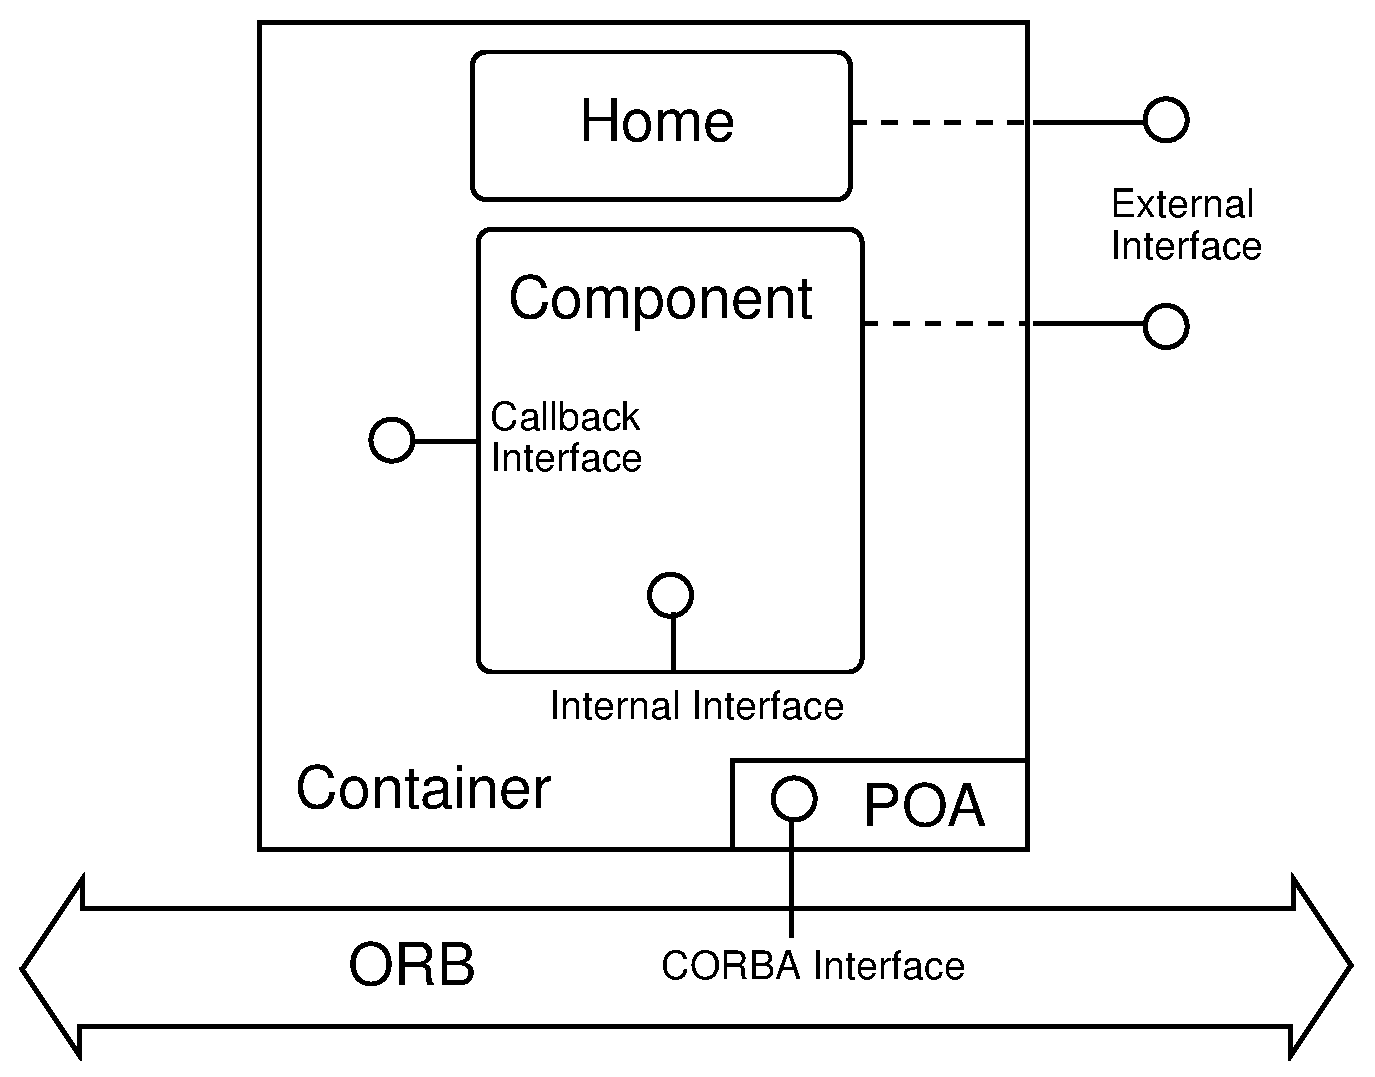
\includegraphics [width=6cm,angle=0] {Container}
        \caption{CCM container}
        \label{container}
    \end{center}
\end{figure}

As shown in Fig.~\ref{container}, the container programming model is made of
interfaces that are used by the client, the container, and the components. These
interfaces fall into the following three categories:

\begin{description}
\item [Internal interfaces]
These local interfaces are used by the component developer and provided by the
container to assist in the implementation of the component's behavior.

\item [External interfaces]
The external interfaces define the external view of a component. They are used
by the client and implemented by the component developer.

\item [Callback interfaces]
These local interfaces are used by the container and implemented by the
component, either in generated code or directly, so that the component can be
deployed in the container.
\end{description}

The CCM specification defines four component categories. The behavior of these
categories is specified by the container interface types. Additionally, there is
a component category that describes the empty container.

\begin{description}
\item [Service component]
The {\it service component} has behavior, no state, and no identity. The
lifespan of a service component is equivalent to the lifetime of a single
operation request.

\item [Session component]
The {\it session component} has behavior, transient state, and an identity
(which is not persistent). Note that the session component is equivalent to the
stateful session bean found in Enterprise Java Beans (EJB).

\item [Process component]
The {\it process component} has behavior, persistent state (which is not visible
to the client), and a persistent identity.

\item [Entity component]
The {\it entity component} has behavior, persistent state (which is visible to
the client), and an identity (which is visible to the clients through a primary
key declaration).
\end{description}

\newpage

%==============================================================================
\section{Component assembly}
%==============================================================================

In component based development, applications are collections of connected component
instances.  
The CCM specification provides a way to form component {\it Assemblies} 
(Fig.~\ref{assemblygraph}) by connecting components through their facets and receptacles.

\begin{figure}[!htb]
    \begin{center}
        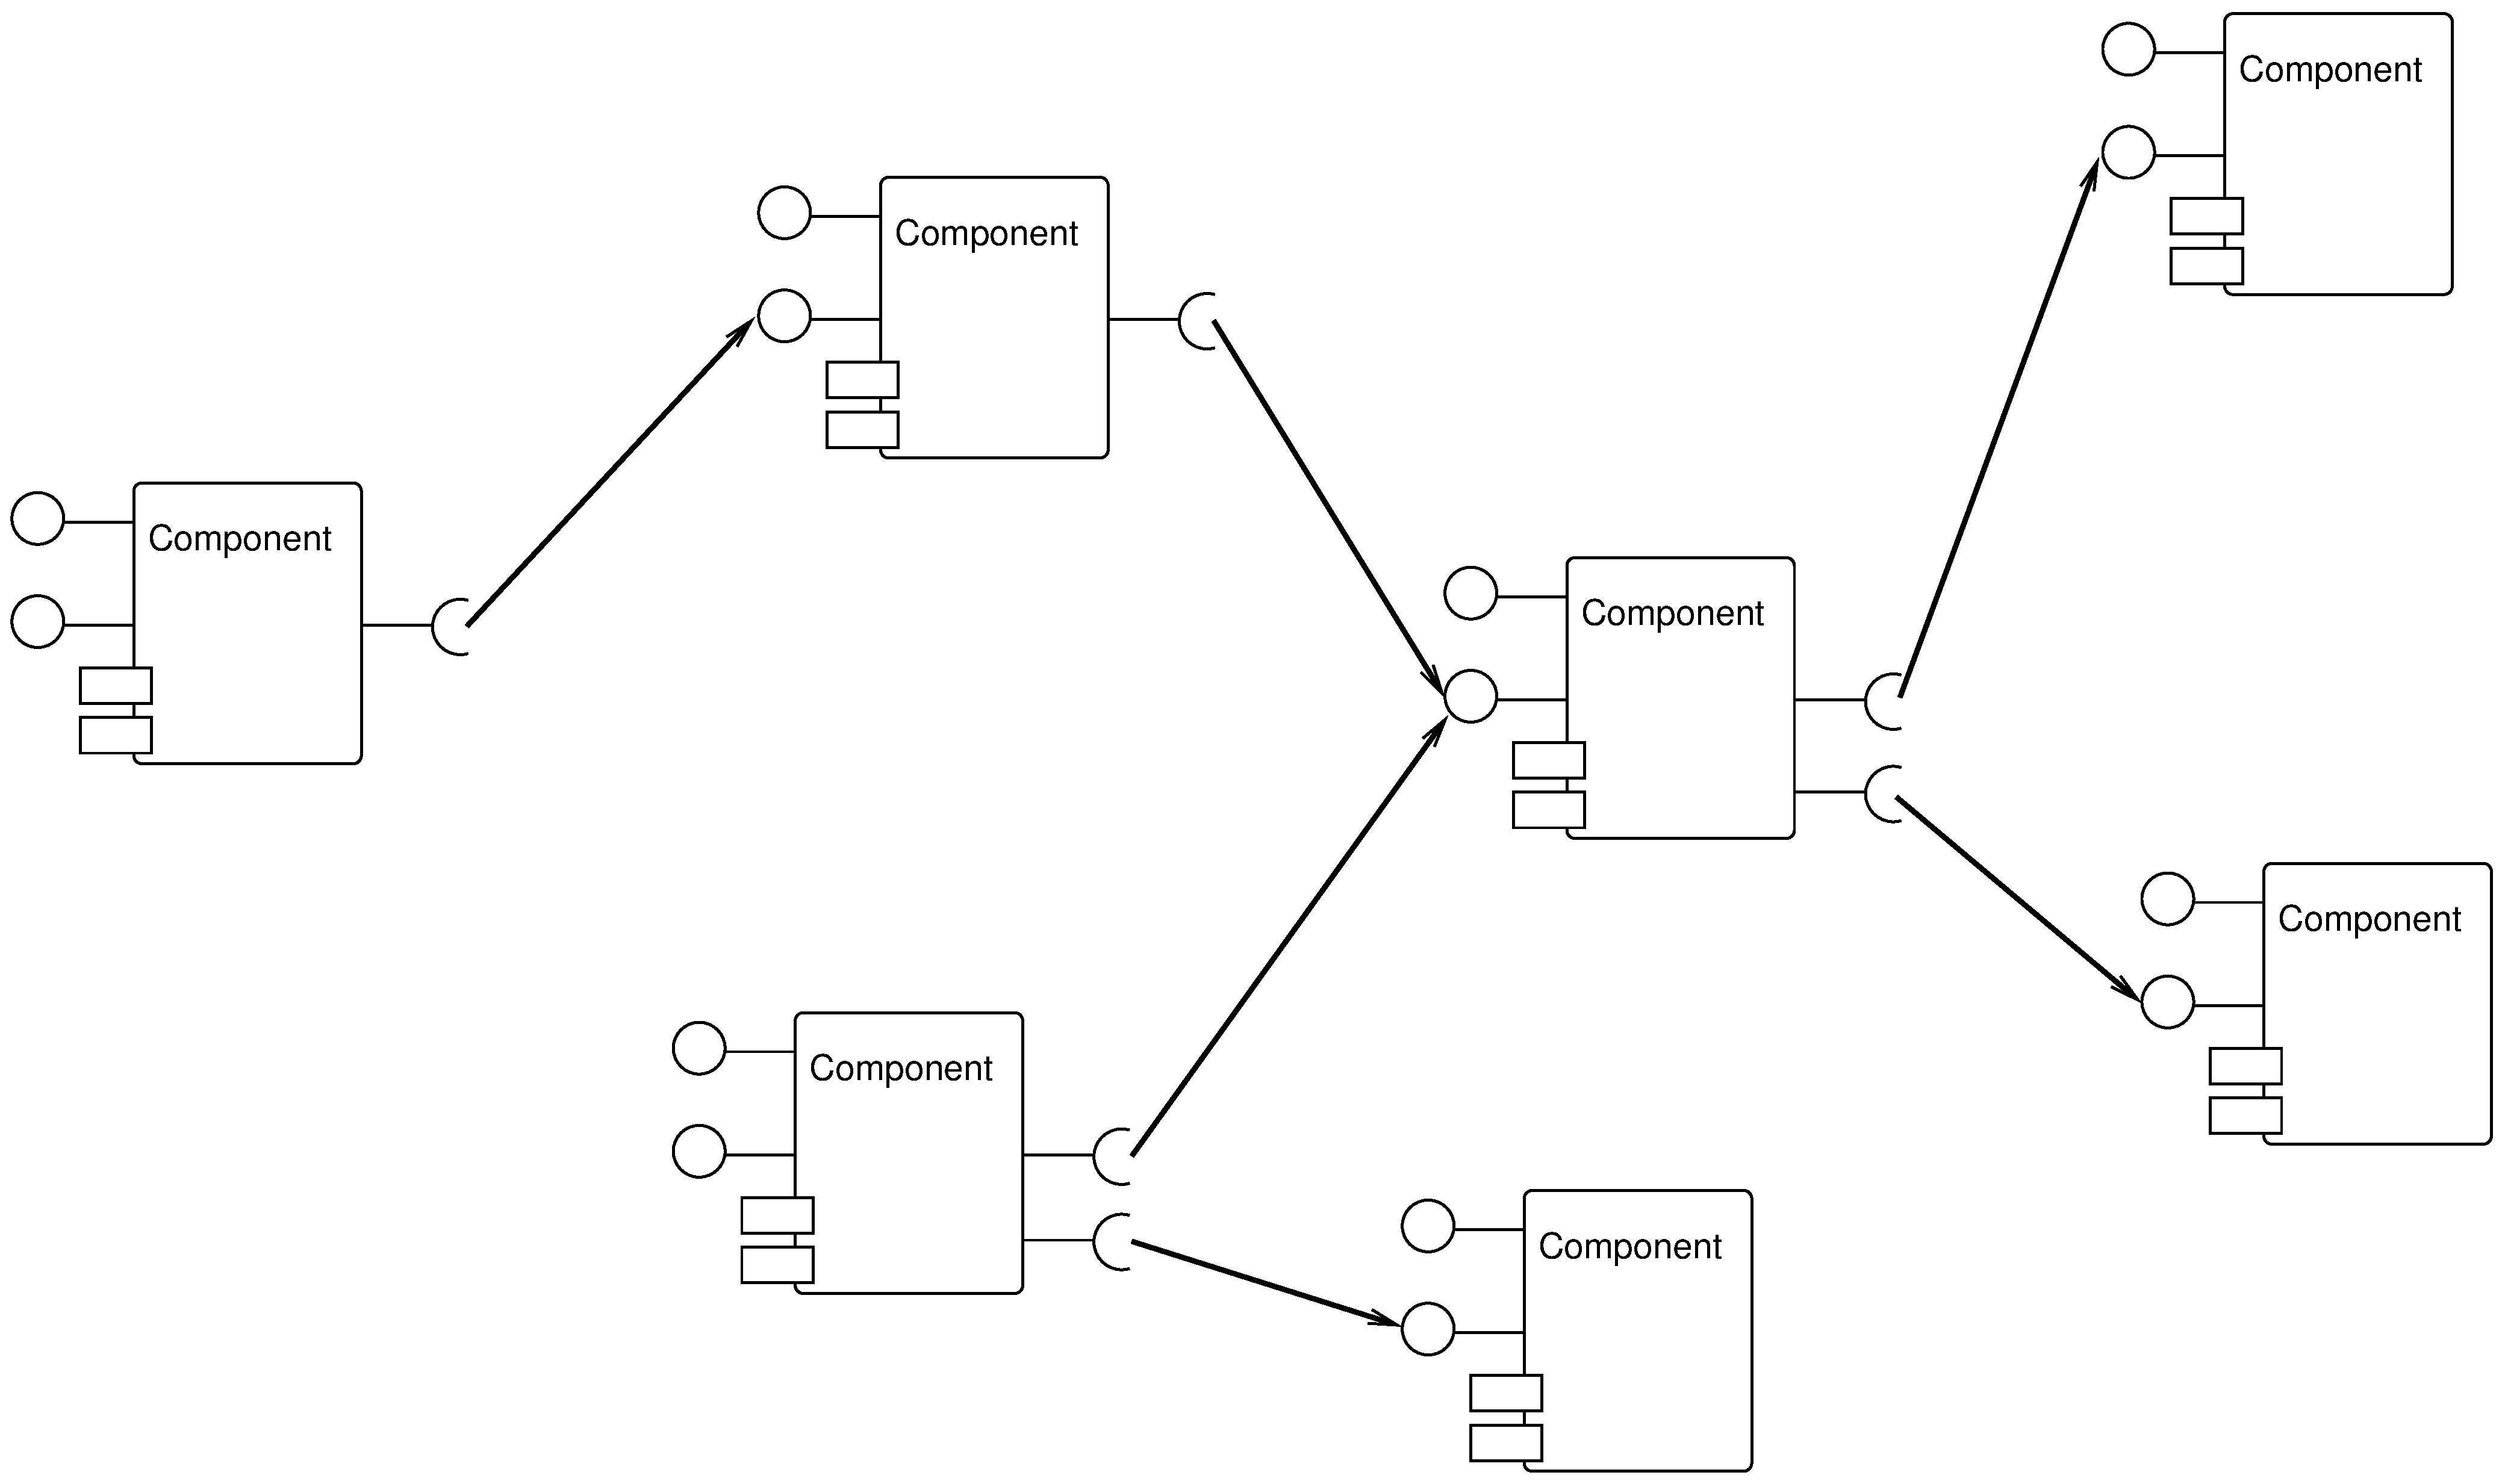
\includegraphics [width=10cm,angle=0] {Assembly}
        \caption{Component assembly}
        \label{assemblygraph}
    \end{center}
\end{figure}

The CCM specification also defines a {\tt Components::Assembly} interface that
represents an assembly instance. It is used to build up and tear down component
assemblies. Building the assembly up means creating all of the necessary
components and establishing connections between them as specified in a file
called the {\it assembly descriptor\/}. Tearing the assembly down means removing
all connections and destroying the components.




%==============================================================================
\section{Client programming model}
%==============================================================================

The client interacts with a CORBA component through two forms of external
interfaces, a home interface and one or more application interfaces. Two forms
of clients are supported by the CCM specification:

\begin{description}
\item [Component--aware client]
This client knows that it is making requests to a component. The client can use
component mechanisms like navigation between components through facets and
receptacles, etc. Component--aware clients locate their interfaces using the
{\tt Components::HomeFinder} or a naming service.

A reference that supports the {\tt HomeFinder} interface may be obtained from
the ORB by invoking {\tt CORBA::ORB::resolve\_initial\_references()} with the
parameter value {\tt ``ComponentHomeFinder''}.

\item [Component--unaware client]
This client does not know that there is a CORBA component. The client requests
are made as if the requests are going to ordinary CORBA objects and object
factories.
\end{description}


\newpage
%==============================================================================
\section{Light Weight CORBA Component Model}
%==============================================================================

Many of today's embedded CORBA applications are unable to use the available 
enterprise CCM due to design constraints.
These constraints include small code size in embedded environments and 
limited processing overhead for performance conservative applications.

To overcome this problem, a {\bf Light Weight CORBA Component Model} (LWCCM)
was submitted to the OMG \cite{LwCCM-Specification}.
The purpose of this profile is to specify a lightweight version of the CCM.
This profile tries to be as compliant as possible to the OMG 
{\bf Minimum CORBA} specification \cite{Minimum_CORBA}.


The principal aim of LWCCM is to have a component model sufficient to compose
applications with CORBA components without all optional features that are
not part of the ``core'' capabilities CCM.
This profile exposes what mandatory features should be contained in a 
minimum implementation of the CCM. 
The choices made in the profile follow rules established to suit embedded
environments:
\begin{itemize}
\item {\bf No Redundancy}:
If several ways of requesting a service exist, only one is retained.

\item {\bf Interoperability and Compatibility with full CCM}:
During deployment, a lightweight component should be deployable by a full
CCM deployment application. Connections between a lightweight component
and a full CCM component must be possible.
Implementations of lightweight components should be source compatible
with the full CCM.

\item {\bf No Persistence}:
The LWCCM does not need to manage any kind of persistence as described in the
CCM specification. 

\item {\bf No Transactions}:
Transactions are not a feature commonly used in embedded systems thus they
are not included in the LWCCM profile.

\item {\bf No Security}:
Security will not be treated in the LWCCM profile.

\item {\bf Less Introspection}:
Not all introspection operations are retained in this profile because they
are not essential to perform the deployment of components.
\end{itemize}

\noindent
The {\it CCM Implementation Framework} (CIF) will use the IDL descriptions and
possibly an XML description file of the component to generate programming skeletons.
The whole chapter concerning CIDL is excluded from the LWCCM profile.
The CIDL is redundant with IDL definitions because all functional descriptions
of the component (facets, receptacles, events and attributes) is done with the IDL files.
The way to assign a component category (service or session) to a component
can be done via an XML description file that will be used with the IDL files to
generate container code and skeletons.


	% $Id$
%==============================================================================
\section{Light Weight CORBA Component Model}
%==============================================================================

Many of today's embedded CORBA applications are unable to use the available 
enterprise CCM due to design constraints.
These constraints include small code size in embedded environments and 
limited processing overhead for performance conservative applications.

\vspace{3mm}
\noindent
To overcome this problem, LwCCM
was submitted to the OMG \cite{LwCCM-Specification}.
The purpose of this profile is to specify a lightweight version of the CCM.
The principal aim of LwCCM is to have a component model sufficient to compose
applications with CORBA components without all optional features that are
not part of the ``core'' capabilities of CCM.
%This profile exposes what mandatory features should be contained in a 
%minimum implementation of the CCM. 
The choices made in the profile follow rules established to suit embedded
environments:
\begin{itemize}
\item {\bf Redundancy.}
If several ways of requesting a service exist, only one is retained.

\item {\bf Interoperability and Compatibility with full CCM.}
During deployment, a leightweight component should be deployable by a full
CCM deployment application. Connections between a leightweight component
and a full CCM component must be possible.
Implementations of leightweight components should be source compatible
with the full CCM.

\item {\bf Persistence.}
The LwCCM does not need to manage any kind of persistence as described in the
CCM specification. 

\item {\bf Transactions.}
Transactions are not a feature commonly used in embedded systems thus they
are not included in the LwCCM profile.

\item {\bf Security.}
Security will not be treated in the LwCCM profile.

\item {\bf Introspection.}
Not all introspection operations are retained in this profile because they
are not essential to perform the deployment of components.

\item {\bf EJB Integration.}
There is no integration of {\it Enterprise JavaBeans} defined in LwCCM
because EJB are not required for embedded targeted environments.

\item {\bf Deployment and Configuration.}
Instead of the {\it Packaging and Deployment} chapter of CCM, LwCCM
is based on the OMG {\it Deployment and Configuration} specification 
\cite{DeploymentAndConfiguration}.
This includes also the definitions of component and assembly descriptor
files and their XML DTDs.

\item {\bf CCM Implementation Framework.}
The whole {\it Component Implementation Definition Language} (CIDL) chapter 
as well as the {\it CCM Implementation Framework} (CIF) chapter are excluded 
from the LwCCM profile.

The CIDL is redundent with IDL definitions because all functional descriptions
of the component (facets, reseptacles, events and attributes) is done with the 
IDL files.
The way to assign a component category (service or session) to a component
can be done via an XML description file that will be used with the IDL files to
generate container code and skeletons.
\end{itemize}

\noindent
This profile tries to be as compliant as possible to the OMG 
{\bf Minimum CORBA} and {\bf Lightweight Services} specifications 
\cite{Minimum_CORBA, LightweightServices}.



%==============================================================================
\end{appendix}


%=References===================================================================
\bibliographystyle{plain}
\bibliography{bibtex/cbse,bibtex/doc,bibtex/wx,bibtex/pattern,bibtex/se,bibtex/mda}
%==============================================================================
\end{document}
